Predikátová logika (PL) pracuje s primitivními formulemi (\textbf{predikáty}) vypovídajícími o \textbf{vlastnostech} a \textbf{vztazích} mezi \textbf{předměty} jistého \textbf{univerza} (individui). Je rozšířením výrokové logiky. Na rozdíl od výrokové logiky si všímá i struktury vět samotných a obsahuje predikáty a kvantifikátory. Pouze jen malá část úsudku může být formalizována pomocí výrokové logiky:

\begin{center}
\begin{minipage}{0.5\textwidth}
Všechny opice mají rády banány
\\
Judy je opice
\resline
Judy má ráda banány
\end{minipage}
\end{center}

Z hlediska VL jsou to jednoduché výroky
$p, q, r$ a z $p, q$ nevyplývá $r$.


\subsection{Predikátová logika 1. řádu}
Predikátová logika umožňuje uvažování nad \textbf{vlastnostmi}, jež jsou \textbf{sdíleny mnoha objekty}, díky použití \textbf{proměnných} a \textbf{kvantifikátorů}. V predikátové logice by byl výše uvedený úsudek formalizován takto:

\begin{center}
\begin{minipage}{0.7\textwidth}
Každé individuum, je-li \textbf{O}pice pak má rádo \textbf{B}anány.\\
{J}udy je individuum s vlastností být \textbf{O}pice.
\resline
\textbf{J}udy je individuum s vlastností mít rádo \textbf{B}anány.
\end{minipage}
\end{center}

$\forall x (O(x) \rightarrow B(x)); O(J) \neq B(J)$, kde x je \textbf{individuová proměnná}; O, B \textbf{predikátové symboly} a J \textbf{funkční symbol}.

\paragraph*{Poznámka} Pokud bychom chtěli formalizovat úsudky, které navíc vypovídají i o vlastnostech vlastností a vztahů a o vztazích mezi vlastnostmi a vztahy, museli bychom použít predikátovou logiku druhého řádu a vyššího. Tou se ale nebudeme zabývat.

\subsubsection{Formální jazyk PL1 -- Abeceda}
\textbf{Logické symboly:}
\begin{itemize}
\item Individuové proměnné: $x, y, z$, \ldots
\item Logické spojky:  $\land$ konjunkce, $\lor$ disjunkce, $ \rightarrow $ implikace,  $ \leftrightarrow $ ekvivalence, $ \lnot $ negace.
\item Kvantifikační symboly: $\forall, \exists$.
\end{itemize}

\noindent\textbf{Speciální symboly:} (n-arita = počet argumentů)
\begin{itemize}
\item Predikátové: $P^n, Q^n$, \ldots
\item Funkční: $f^n, g^n, h^n$, \ldots
\end{itemize}

\noindent\textbf{Pomocné symboly:} závorky a jiná interpunkční znaménka (, ), \ldots

\subsubsection{Formální jazyk PL1 -- Gramatika}
\textbf{Termy:}
\begin{enumerate}
\item každý symbol proměnné $x, y$, \ldots je \textbf{term},
\item jsou-li $ t_1, \ldots, t_n $ ($n \geq 0$) termy a je-li $f$ n-ární \textbf{funkční symbol}, pak výraz $f(t_1, \ldots, t_n)$ je term; pro $n = 0$ se jedná o \textbf{individuovou konstantu} (značíme $a, b, c, \ldots$),
\item jen výrazy dle 1. a 2. jsou termy.
\end{enumerate}

\noindent\textbf{Atomické formule:}
\begin{itemize}
\item je-li $ P $ n-ární predikátový symbol a jsou-li $ t_1, \ldots, t_n $ termy, pak výraz $ P(t_1, \ldots, t_n) $ je \textbf{atomická formule} (na vstupu jsou pouze termy).
\end{itemize}

\noindent\textbf{Formule:}
\begin{itemize}
\item každá atomická formule je formule,
\item je-li výraz $ A $ formule, pak $\neg A$ je formule,
\item jsou-li výrazy $A$ a $B$ formule, pak výrazy $(A \land B), (A \lor B), (A \rightarrow B), (A \leftrightarrow B)$ jsou formule, je-li $ x $ proměnná a $A$ formule, pak výrazy $\forall x A$ a $\exists x A$ jsou formule.
\end{itemize}

\subsection{Převod z přirozeného jazyka do PL1}
\begin{itemize}
\item $\forall$ -- ,,všichni'', ,,žádný'', ,,nikdo'', \ldots
\item $\exists$ --  ,,někdo'', ,,něco'', ,,někteří'', ,,existuje'', \ldots
\end{itemize}

\noindent Větu musíme často ekvivalentně přeformulovat, pozor: v češtině \textbf{dvojí zápor}!
\begin{itemize}
\item Žádný student není důchodce: $\forall x (S(x) \rightarrow \neg D(x))$.
\item Ale, ,,všichni studenti nejsou důchodci'' čteme jako ,,ne všichni studenti jsou důchodci'': 
$\neg \forall x (S(x) \rightarrow D(x)) \leftrightarrow x (S(x) \rightarrow \neg D(x))$
\end{itemize}

\noindent Jako \textbf{pomůcka} k řešení může sloužit tato zásada:
\begin{itemize}
\item Po \textbf{všeobecném} kvantifikátoru následuje formule ve tvaru implikace: $\forall \ldots \rightarrow$.
\item Po \textbf{existenčním} kvantifikátoru formule ve tvaru konjunkce:  $\exists \ldots \land$.
\end{itemize}

\subsubsection{Volné a vázané proměnné}
\begin{figure}[H]
	\centering
	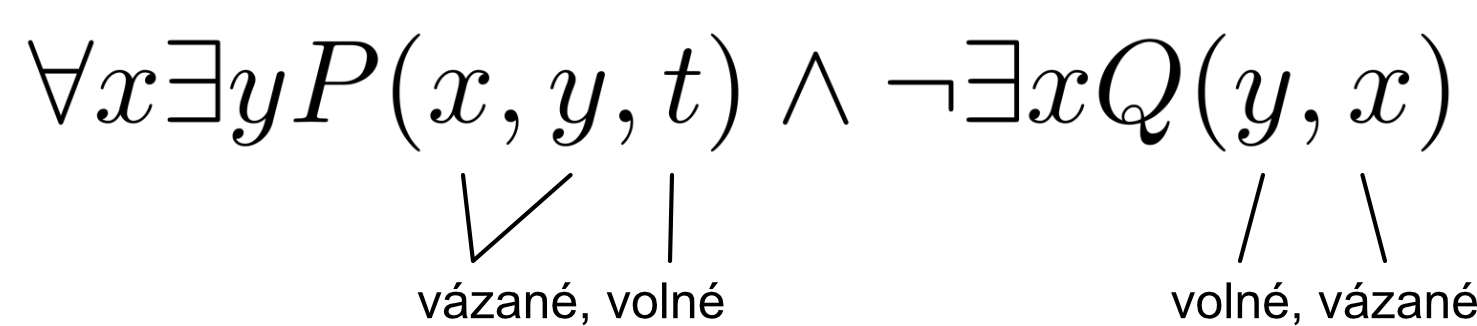
\includegraphics[width=.6\textwidth]{assets/volne_vazane}
\end{figure}

\subsection{Ekvivalentní úpravy}
Při ekvivalentních úpravách se používají \textbf{de Morganovy} zákony v PL1: $\neg \forall xA \leftrightarrow \exists x\neg A$ \qquad $\neg \exists xA \leftrightarrow \forall x\neg A$.

\subsubsection*{Příklady}
\begin{itemize}
\item Není pravda, že všichni vodníci jsou zelení. $ \leftrightarrow $ Někteří vodníci nejsou zelení.\\$\neg{}\forall{}x (V(x) \rightarrow Z(x)) \leftrightarrow \exists{}x (V(x) \land \neg{}Z(x))$
\item Není pravda, že někteří vodníci jsou zelení. $ \leftrightarrow $ Žádný vodník není zelený.\\
$\neg{}\exists{}x (V(x) \land Z(x)) \leftrightarrow \forall{}x (V(x) \rightarrow \neg{}Z(x))$
\item Everybody loves somebody sometimes.\\
$\forall{}x \forall{}y \forall{}z L(x,y,z)$
\item Marie má ráda pouze vítěze.\\
$\forall{}x (R(m,x) \rightarrow V(x))$
\end{itemize}

\subsection{Ekvivalentní transformace}
\begin{itemize}
	\item Aplikace negace: $\neg{}\forall{}x [V(x) \rightarrow{} Z(x)] \quad \leftrightarrow \quad \exists{}x [V(x) \land{} \neg{}Z(x)]$.
	\item \textbf{De morganovy} zákony: $\forall{}x [((P(x) \land{}Q(x)) \lor{}D(x)] \quad \leftrightarrow \quad \forall{}x [(P(x) \lor{}D(x)) \land{}(Q(x) \lor{}D(x))]$.
	\begin{itemize}
		\item[] $\neg (A\vee B)\iff (\neg A)\wedge (\neg B)$
		\item[] $\neg (A\wedge B)\iff (\neg A)\vee (\neg B)$
	\end{itemize}
	\item Převod \textbf{implikace}: $\forall{}x (P(x) \rightarrow{}G(x)) \quad \leftrightarrow \quad \forall{}x (\neg{}P(x)\lor{}G(x))$.
\end{itemize}

\noindent Patří zde i část z převodu do \textbf{Skolemovy Klauzární formy}:
\begin{enumerate}
\item eliminace nadbytečných kvantifikátorů,
\item eliminace spojek $\rightarrow, \leftrightarrow$,
\item přesun negace dovnitř,
\item přejmenování proměnných,
\item přesun kvantifikátorů doprava,
\item přesun všeobecných kvantifikátorů doleva,
\item použití distributivních zákonů.
\end{enumerate}

\subsection{Sémantika v PL1}
\begin{itemize}
\item Při substituci termů za proměnné (A(x/t)), je třeba dbát na nahrazování pouze \textbf{volných proměnných}.
\item Při definici formule, je nutné vysvětlit co \textbf{znamenají} jednotlivé predikátové symboly, termy atd.
\end{itemize}

